%!TEX root = ../aluno.tex

\chapter{Folhas para reprodução}

\section*{Lição 1}

\setcounter{atividade}{0}
%atividade 1
\begin{atividade}
\vspace{.2cm}

\begin{center}
\begin{tikzpicture}[scale=21]
 \draw[fill=chocolate] (0,0) rectangle (4.5,2);
\end{tikzpicture}


\begin{tikzpicture}[scale=21]
 \draw[fill=chocolate] (0,0) rectangle (4.5,2);
 \draw (1,0) -- (1,2);
 \draw (2.5,0) -- (2.5,2);
\end{tikzpicture}
\end{center}
\end{atividade}

%atividade 2
\begin{atividade}
\centering
\includegraphics[width=.95\linewidth]{reproducao/licao01-ativ02.png}
\end{atividade}

\clearpage

%atividade 3
\begin{atividade}
\begin{center}
\begin{tikzpicture}[scale=10]
\fill[attention]  \foreach \x/\y in {36/72,108/144,180/212, 252/284, 324/360}{ (0,0) -- (\x-18:4) -- (\y-18:2)--(\x-18 +72:4) -- (0, 0)};
\draw  \foreach \x/\y in {36/72,108/144,180/212, 252/284, 324/360}{ (\x-18:4) -- (\y-18:2)--(\x-18 +72:4)};
\end{tikzpicture}
\end{center}
\end{atividade}

\begin{atividade}
\centering
 \begin{tikzpicture}[scale=1.25, x=1cm,y=1cm]
  \draw (0,0) rectangle (1,6);
  \draw (1,0) rectangle (2,6);
  \draw (2,0) rectangle (3,6);
  \draw (3,0) rectangle (4,6);
  \draw (5,0) rectangle (9,3);
  \draw (5,0) rectangle (9,6);
  \draw (5,0) -- (9,3);
  \draw (5,3) -- (9,6);
\end{tikzpicture}
\clearpage

\null
\vfill
\begin{tikzpicture}[scale=1.25, x=1cm,y=1cm]
  \draw (0,0) rectangle (4,1.5);
  \draw (0,1.5) rectangle (4,3);
  \draw(0,3) rectangle (4,4.5);
  \draw(0,4.5) rectangle (4,6);
  \draw(5,0) rectangle (9,3);
  \draw(5,0) rectangle (9,6);
  \draw(7,0) -- (7,6);
\end{tikzpicture}


 \begin{tikzpicture}[scale=1.25, x=1cm,y=1cm]
  \draw (10,0) rectangle (14,3);
  \draw (10,3) rectangle (14,6);
  \draw(12,0) -- (12,3);
  \draw(10,4.5) -- (14,4.5);
  \draw(15,0) rectangle (19,3);
  \draw(15,3) rectangle (19,6);
  \draw(15,1.5) -- (19,1.5);
  \draw(15,3) -- (19,6);
\end{tikzpicture}
\vspace{0.5cm}

\begin{tikzpicture}[scale=1.25, x=1cm,y=1cm]
  \draw (10,0) rectangle (14,3);
  \draw (10,3) rectangle (14,6);
  \draw (12,0) -- (12,3);
  \draw (10,3) -- (14,6);
  \draw (15,0) rectangle (19,3);
  \draw (15,3) rectangle (19,6);
  \draw (15,0) -- (19,3);
  \draw (19,3) -- (15,6);
\end{tikzpicture}
\vfill
\null
\end{atividade}
\clearpage

\setcounter{atividade}{9}

%Atividade 10
\begin{atividade}
%retângulos
\begin{center}
\resizebox{.7\linewidth}{!}
{
\begin{tikzpicture}[scale=2, x=1cm,y=1cm]
 \draw[fill=bwattention] (0,0) rectangle (3,2);
 \draw (3,0) rectangle (6,2) (3,-0.4) node{Figura 1};
\end{tikzpicture}
}

\resizebox{.7\linewidth}{!}
{
\noindent\begin{tikzpicture}[scale=2, x=1cm,y=1cm]
 \draw (0,0) rectangle (3,2);
 \draw (1,0) -- (1,2);
 \draw (1.5,0) -- (1.5,2);
 \draw (2.2,0) -- (2.2,2);
 \draw[fill=bwattention] (3,0) rectangle (6,2) (3,-0.4) node{Figura 2};
\end{tikzpicture}
}

\resizebox{.7\linewidth}{!}
{
\noindent\begin{tikzpicture}[scale=2, x=1cm,y=1cm]
 \draw (0,0) rectangle (3,2);
 \draw (3,0) rectangle (6,2) (3,-0.4) node{Figura 3};
 \draw[fill=bwattention] (0,2) rectangle (6,1.2);
 \end{tikzpicture}
}
\end{center}
\clearpage

 % círculos

\resizebox{\linewidth}{!}
{
\begin{tikzpicture}[scale=2, x=1cm,y=1cm]
 \draw[fill=bwattention] (0,-2) arc (-90:90: 2);
 \draw (0,2) arc (90:270:2) (0,-2.4) node{Figura 4};
\end{tikzpicture}
\begin{tikzpicture}[scale=2, x=1cm,y=1cm]
 \draw[fill=bwattention] (45:2) arc (45:225:2);
 \draw (225:2) arc (225:405:2) (0,-2.4) node{Figura 5};
 \draw (0,0) -- (0,-2);
 \draw (0,0) -- (-30:2);
 \draw (225:2) -- (45:2);
 \end{tikzpicture}
}

\resizebox{\linewidth}{!}
{
 \begin{tikzpicture}[scale=2, x=1cm,y=1cm]
 \draw (0,0) circle (2);
 \draw[fill=bwattention] (0,0) -- (2,0) arc (0:90:2) -- cycle;
 \draw[fill=bwattention] (0,0) -- (-2,0) arc (180:270: 2) -- cycle;
 \node at (0,-2.4) {Figura 6};
\end{tikzpicture}
\begin{tikzpicture}[scale=2, x=1cm,y=1cm]% hexágonos
 \foreach \x in {0,60,...,300}{
 \draw (\x:2) -- (\x +60: 2);}
 \fill[bwattention] (2,0) -- (60:2) -- (300:2);
 \node at (0,-2.4) {Figura 7};
\end{tikzpicture}
}
\clearpage

\resizebox{\linewidth}{!}
{
\begin{tikzpicture}[scale=2, x=1cm,y=1cm]
 \foreach \x in {0,60,...,300}{
 \draw (\x:2) -- (\x +60: 2);}
 \fill[bwattention] (60:2) -- (120:2) -- (180:2) -- (240:2) --cycle;
 \draw (0,0) -- (2,0);
 \draw (0,0) -- (300:2) (0,-2.4) node{Figura 8};
\end{tikzpicture}
\begin{tikzpicture}[scale=2, x=1cm,y=1cm]
 \foreach \x in {0,60,...,300}{
 \draw (\x:2) -- (\x +60: 2);}
 \fill[bwattention] (0:2) -- (60:2) -- (0:0) --cycle;
 \fill[bwattention] (120:2) -- (180:2) -- (0:0) --cycle;
 \fill[bwattention] (240:2) -- (300:2) -- (0:0) --cycle;
 \node at (0,-2.4) {Figura 9};
\end{tikzpicture}
}

%círculo

\resizebox{\linewidth}{!}
{
\begin{tikzpicture}[scale=2, x=1cm,y=1cm]
 \draw[fill=bwattention] (0:2) arc (0:270:2) -- (0,0) -- cycle;
 \draw (270:2) arc (270:360:2);
 \draw (0,0) -- (0,-2);
 \draw (0,0) -- (2,0)  (0,-2.4) node{Figura 10};
 \end{tikzpicture}
\begin{tikzpicture}[scale=2, x=1cm,y=1cm]%hexágonos
 \foreach \x in {0,60,...,300}{
 \draw (\x:2) -- (\x +60: 2);}
\fill[bwattention] (120:2) -- (180:2) -- (240:2) -- cycle;
\fill[bwattention] (240:2) -- (300:2) -- (60:2) -- cycle;
 \node at (0,-2.4) {Figura 11};
\end{tikzpicture}
}

%retângulo
\begin{center}
\resizebox{.7\linewidth}{!}
{
\begin{tikzpicture}[scale=2, x=1cm,y=1cm]
 \fill[bwattention] (1,0) rectangle (4,2);
 \draw (0,0) rectangle (6,2);
 \node at (3,-0.4) {Figura 12};
 \end{tikzpicture}
}
\end{center}

\end{atividade}
\clearpage

% Atividade 11
\begin{atividade}

\resizebox{\linewidth}{!}
{
 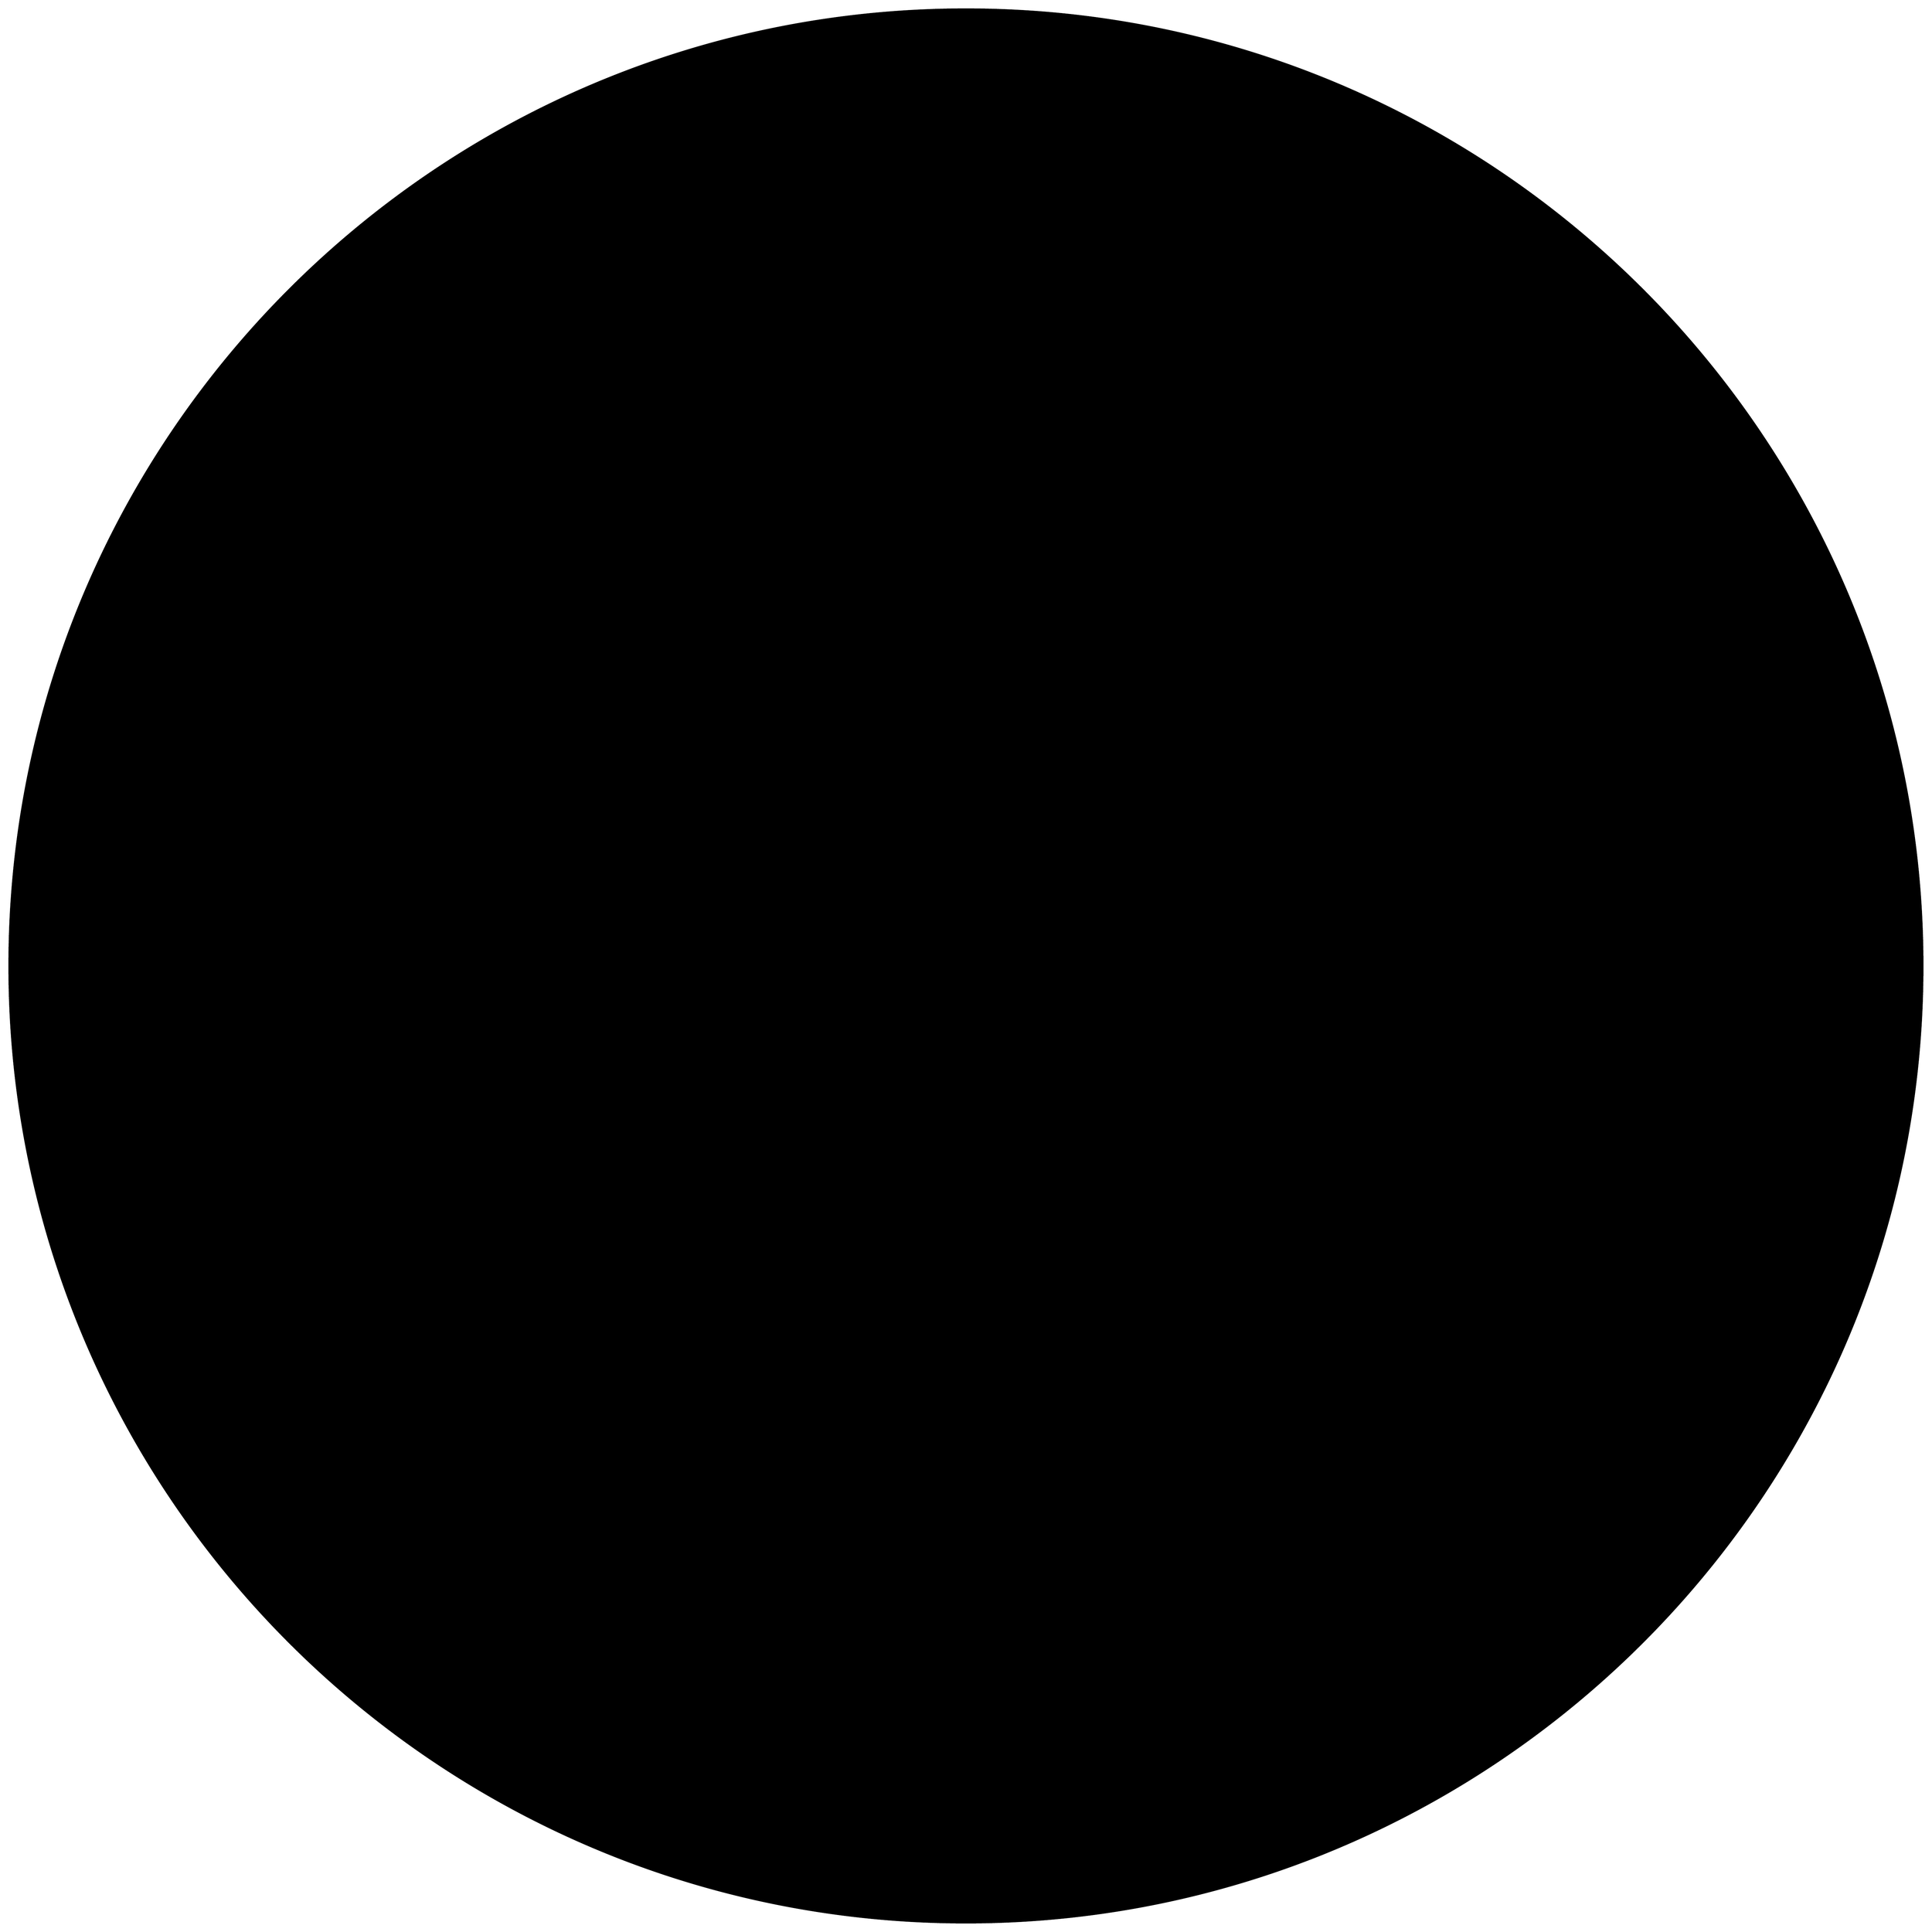
\begin{tikzpicture}
\fill[black] (0,0) circle (40);
 \end{tikzpicture}
\begin{tikzpicture}
\fill[cbpink] (0,0) circle (40);
\draw[line width =.25mm, white] (-90:40) -- (90:40);
\end{tikzpicture}
}

 \resizebox{\linewidth}{!}
 {
 \begin{tikzpicture}
 \fill[common] (0,0) circle (40);
 \foreach \x in {30,150,270} \draw[line width =.25mm, white] (0,0)--(\x:40);
 \end{tikzpicture}
  \begin{tikzpicture}
 \fill[attention] (0,0) circle (40);
 \foreach \x in {0,90} \draw[line width =.25mm, white] (\x:-40)--(\x:40);
 \end{tikzpicture}
 }

\resizebox{\linewidth}{!}
{
 \begin{tikzpicture}
\fill[cbolive] (0,0) circle (40);
\foreach \x in {18,90,...,360} \draw[line width =.25mm, white] (0,0)--(\x:40);
\end{tikzpicture}
\begin{tikzpicture}
\fill[cbpurple] (0,0) circle (40);
\foreach \x in {0,60,...,360} \draw[line width =.25mm, white] (0,0)--(\x:40);
\end{tikzpicture}
}

\clearpage

\resizebox{\linewidth}{!}
{
\begin{tikzpicture}
\fill[cbyellow] (0,0) circle (40);
\foreach \x in {0,45,...,360} \draw[line width =.25mm, white] (0,0)--(\x:40);
\end{tikzpicture}
\begin{tikzpicture}
\fill[cbgray] (0,0) circle (40);
\foreach \x in {0,36,...,360} \draw[line width =.25mm, white] (0,0)--(\x:40);
\end{tikzpicture}
}

\resizebox{\linewidth}{!}
{
\begin{tikzpicture}
\fill[cborange] (0,0) circle (40);
\foreach \x in {0,40,...,360} \draw[line width =.25mm, white] (0,0)--(\x:40);
\end{tikzpicture}
\begin{tikzpicture}
\draw (0,0) circle (40);
\foreach \x in {0,36,...,360} \draw[line width =.25mm] (0,0)--(\x:40);
\end{tikzpicture}
}

\end{atividade}
\clearpage

\setcounter{atividade}{12}
% Atividade 13
\begin{atividade}
\resizebox{\linewidth}{!}
{\begin{tikzpicture}[scale=2, x=1cm,y=1cm] %a)
 \draw (0,0) rectangle (4,2);
 \fill[bwattention] (0,0) -- (4,2) -- (4,0) -- cycle;
\end{tikzpicture}
\begin{tikzpicture}[scale=2, x=1cm,y=1cm] %b)
 \draw (0,0) rectangle (4,2);
 \foreach \n in {0.4,0.8,1.2,...,3.2,3.6}{
 \draw (\n,0) -- (\n,2);}
 \fill[bwattention] (0.8,0) -- (0.8,2) -- (1.2,2) -- (1.2,0) -- cycle;
\end{tikzpicture}}

\resizebox{\linewidth}{!}
{
\begin{minipage}{.49\linewidth}
\null\vfill
\resizebox{\linewidth}{!}
{
\begin{tikzpicture}[scale=2, x=1cm,y=1cm] %c)
 \draw (0,0) rectangle (4,2);
 \fill[bwattention] (2,1) rectangle (4,2);
 \draw (0,1) -- (4,1);
 \draw (2,0) -- (2,2);
 \end{tikzpicture}
}\vfill\null
\end{minipage}
\begin{minipage}{.49\linewidth}
\resizebox{\linewidth}{!}
{
\begin{tikzpicture}[scale=2, x=1cm,y=1cm] %d)
 \fill[bwattention] (45:2) arc (45:135:2) -- (0,0) -- cycle;
 \draw (135:2) arc (135:405:2);
\end{tikzpicture}
}
\end{minipage}
}

\resizebox{\linewidth}{!}
{
\begin{minipage}{.49\linewidth}
\resizebox{\linewidth}{!}
{
\begin{tikzpicture}[scale=2,x=1cm,y=1cm] %e)
 \foreach \x in {0,60,...,300}{
 \draw (\x:2) -- (\x +60: 2);}
\fill[bwattention] (-2,0) -- (0,0) -- (0,1.73) -- (120:2) -- cycle;
\end{tikzpicture}
}
\end{minipage}
\begin{minipage}{.49\linewidth}
\null\vfill
\resizebox{\linewidth}{!}
{
\begin{tikzpicture}[scale=2,x=1cm,y=1cm] %f)
 \draw (0,0) rectangle (5,1);
 \draw[fill=bwattention] (0,1) rectangle (5,2);
\end{tikzpicture}
}\vfill\null
\end{minipage}
}

\clearpage

\resizebox{\linewidth}{!}
{
\begin{minipage}{.49\linewidth}
\centering
\null\vfill
\resizebox{!}{!}
{
\begin{tikzpicture}[scale=2,x=1cm,y=1cm] %g)
 \draw[fill=bwattention] (0,0) rectangle (2,1);
 \draw (0,1) rectangle (2,3);
\end{tikzpicture}
}\vfill\null
\end{minipage}
\begin{minipage}{.49\linewidth}
\resizebox{\linewidth}{!}
{
\begin{tikzpicture}[scale=2,x=1cm,y=1cm] %h)
 \draw[fill=bwattention] (200:2) arc (200:236:2) -- (0,0) -- cycle;
 \draw (236:2) arc (236:560:2);
\end{tikzpicture}
}
\end{minipage}
}


\begin{minipage}{.49\linewidth}
\null\vfill
\resizebox{\linewidth}{!}
{
\begin{tikzpicture}[scale=2,x=1cm,y=1cm] %i)
 \draw[line width=2pt] (-1,0) arc (180:270:1);
 \draw (0,-1) arc (270:360:1) -- (1,0) arc (180:0:1);
 \end{tikzpicture}
}
\vfill\null
\end{minipage}
\begin{minipage}{.49\linewidth}
\null\vfill
\resizebox{\linewidth}{!}
{
\begin{tikzpicture} %j)
\tikzset{
  annotated cuboid/.pic={
    \tikzset{%
      every edge quotes/.append style={midway, auto},
      /cuboid/.cd,
      #1
    }
    \draw [every edge/.append style={pic actions, densely dashed, opacity=0}, pic actions]
    (0,0,0) coordinate (o) -- ++(-\cubescale*\cubex,0,0) coordinate (a) -- ++(0,-\cubescale*\cubey,0) coordinate (b) edge coordinate [pos=1] (g) ++(0,0,-\cubescale*\cubez)  -- ++(\cubescale*\cubex,0,0) coordinate (c) -- cycle
    (o) -- ++(0,0,-\cubescale*\cubez) coordinate (d) -- ++(0,-\cubescale*\cubey,0) coordinate (e) edge (g) -- (c) -- cycle
    (o) -- (a) -- ++(0,0,-\cubescale*\cubez) coordinate (f) edge (g) -- (d) -- cycle;
 },
  /cuboid/.search also={/tikz},
  /cuboid/.cd,
  width/.store in=\cubex,
  height/.store in=\cubey,
  depth/.store in=\cubez,
  units/.store in=\cubeunits,
  scale/.store in=\cubescale,
  width=100,
  height=100,
  depth=100,
  units=cm,
  scale=.1,
  x=1mm,y=1mm
}
    \draw[dotted] (2.95,-1.9) -- (25.5,-1.9);
    \pic [fill=bwattention, fill opacity=.8] at (0,0) {annotated cuboid={width=25, height=50, depth=8}};
    \pic at (22.5,0) {annotated cuboid={width=225, height=50, depth=8}};
\end{tikzpicture}
}
\vfill\null
\end{minipage}


\resizebox{.99\linewidth}{!}
{
\begin{tikzpicture}[scale=2,x=1cm,y=1cm] %l)
 \draw[fill=bwattention] (0,2) rectangle (2,4);
 \draw (0,0) rectangle (2,2);
 \draw (2,0) rectangle (4,2);
 \draw (2,2) rectangle (4,4);
 \end{tikzpicture} 
 \hspace{5pt}
 \begin{tikzpicture}[scale=2,x=1cm,y=1cm] %m)
 \fill[bwattention] (1,0) rectangle (2,1);
 \fill[bwattention] (3,0) rectangle (4,1);
 \fill[bwattention] (0,1) rectangle (1,2);
 \fill[bwattention] (2,1) rectangle (3,2);
 \fill[bwattention] (1,2) rectangle (2,3);
 \fill[bwattention] (3,2) rectangle (4,3);
 \fill[bwattention] (0,3) rectangle (1,4);
 \fill[bwattention] (2,3) rectangle (3,4);
 \draw (0,0) rectangle (4,4);
\end{tikzpicture}
}
\end{atividade}
\clearpage

\section*{Lição 2}
%atividade 1
\setcounter{atividade}{0}
\begin{atividade}
\begin{center}

\begin{tikzpicture}[scale=2]
\draw[fill=gray] (0,0) rectangle (60,20);
\end{tikzpicture}
\end{center}
\end{atividade}

%atividade 2
\begin{atividade}
\begin{center}
\begin{tikzpicture}[scale=2]
  \draw (0,0) rectangle (60,30);
 \end{tikzpicture}
\end{center}
\end{atividade}

%
% \subsection*{Atividade 17}
% \vspace{.2cm}
%
% \begin{tikzpicture}%[scale=.5]
% \draw[fill=gray] (0,0) rectangle (60,12);
%     \end{tikzpicture}
%
% \begin{tikzpicture}%[scale=.5]
% \draw[fill=light] (0,0) rectangle (60,12);
% \draw (30,0) -- (30,12);
% \node at (15,6) {{\small $\frac{1}{2}$}};
% \node at (45,6) {{\small $\frac{1}{2}$}};
% \end{tikzpicture}
%
%    \begin{tikzpicture}%[scale=.5]
% \draw[fill=pink] (0,0) rectangle (60,12);
% \foreach \x in {1,2} \draw (\x*60/3,0) -- (\x*60/3,12);
%     \end{tikzpicture}
%
%       \begin{tikzpicture}%[scale=.5]
% \draw[fill=special] (0,0) rectangle (60,12);
% \foreach \x in {1,2,3} \draw (\x*60/4,0) -- (\x*60/4,12);
%     \end{tikzpicture}
%
%    \begin{tikzpicture}%[scale=.5]
% \draw[fill=attention] (0,0) rectangle (60,12);
% \foreach \x in {1,...,4} \draw (\x*60/5,0) -- (\x*60/5,12);
%     \end{tikzpicture}
%
%    \begin{tikzpicture}%[scale=.5]
% \draw[fill=common] (0,0) rectangle (60,12);
% \foreach \x in {1,...,5} \draw (\x*60/6,0) -- (\x*60/6,12);
%     \end{tikzpicture}
%
%     \begin{tikzpicture}%[scale=.5]
% \draw[fill=CornflowerBlue] (0,0) rectangle (60,12);
% \foreach \x in {1,...,6} \draw (\x*60/7,0) -- (\x*60/7,12);
%     \end{tikzpicture}
%
%    \begin{tikzpicture}%[scale=.5]
% \draw[fill=dark] (0,0) rectangle (60,12);
% \foreach \x in {1,...,7} \draw (\x*60/8,0) -- (\x*60/8,12);
%     \end{tikzpicture}
%
%    \begin{tikzpicture}%[scale=.5]
% \draw[fill=Fuchsia] (0,0) rectangle (60,12);'
% \foreach \x in {1,...,8} \draw (\x*60/9,0) -- (\x*60/9,12);
%     \end{tikzpicture}
%
%  \begin{tikzpicture}%[scale=.5]
%  \draw[fill=NavyBlue] (0,0) rectangle (60,12);
%  \foreach \x in {1,...,9} \draw (\x*60/10,0) -- (\x*60/10,12);
%      \end{tikzpicture}
%
% \begin{tikzpicture}%[scale=.5]
%     \draw[fill=BlueViolet] (0,0) rectangle (60,12);
% \foreach \x in {1,...,15} \draw (\x*60/16,0) -- (\x*60/16,12);
%     \end{tikzpicture}
%

\section*{Lição 3}

%atividade 6
\setcounter{atividade}{5}
\begin{atividade}
\begin{center}
\begin{tikzpicture}[x=115mm,y=115mm]
\draw[fill=common] (0,-.15) rectangle (1.2,.15);
\draw (0,0) -- (1.2,0) ; %edit here for the axis
\draw (1,3pt) -- (1,-3pt) node[below] {1};
\node at (.03,-.05) {0};
\end{tikzpicture}
\end{center}
\end{atividade}
\clearpage

%atividade 7
\begin{atividade}
\begin{center}
\begin{tikzpicture}
 \draw[fill=gray] (0,0) rectangle (110,15);
\end{tikzpicture}
\end{center}
\end{atividade}

\section*{Lição 4}

\setcounter{atividade}{1}

%atividade 2
\begin{atividade}
\begin{center}
\begin{tikzpicture}[scale=1.5]
 \fill[gray] (0,0) rectangle (80,18);
 \draw (0,0) rectangle (80,60);
 \foreach \x in {6,12,...,54} \draw (0,\x) -- (80,\x);
\end{tikzpicture}
\end{center}
\end{atividade}
\clearpage

\setcounter{atividade}{3}

%atividade 4
\begin{atividade}
\resizebox{.99\linewidth}{!}
{
\begin{tikzpicture}
\draw (0,0) circle (40);
\foreach \x in {30,150,270} \draw[line width =1mm] (0,0)--(\x:40);
\end{tikzpicture}
\begin{tikzpicture}
\draw (0,0) circle (40);
\foreach \x in {30,60,...,360} \draw[line width =.2mm] (0,0)--(\x:40);
\draw[line width =1mm] (0,0)--(0:40);
\draw[line width =1mm] (0,0)--(120:40);
\draw[line width =1mm] (0,0)--(240:40);
\end{tikzpicture}
}
\end{atividade}

%atividade 5
\begin{atividade}
\begin{center}
 \begin{tikzpicture}[scale=2.8]
  \draw[fill=gray] (20,0) arc (0:240:20) -- (0,0)--cycle;
  \draw (0,0) circle (20);
 \end{tikzpicture}
\end{center}
\end{atividade}
\clearpage

%atividade 6
\begin{atividade}
\begin{center}
\begin{tikzpicture}[scale=2]
\draw[fill=cborange] (0,0) rectangle (60,12);
\draw (30,0) -- (30,12);
    \end{tikzpicture}

   \begin{tikzpicture}[scale=2]
\draw[fill=cbpink] (0,0) rectangle (60,12);
\foreach \x in {1,2} \draw (\x*60/3,0) -- (\x*60/3,12);
    \end{tikzpicture}

      \begin{tikzpicture}[scale=2]
\draw[fill=attention] (0,0) rectangle (60,12);
\foreach \x in {1,2,3} \draw (\x*60/4,0) -- (\x*60/4,12);
    \end{tikzpicture}

   \begin{tikzpicture}[scale=2]
\draw[fill=stred] (0,0) rectangle (60,12);
\foreach \x in {1,...,4} \draw (\x*60/5,0) -- (\x*60/5,12);
    \end{tikzpicture}

   \begin{tikzpicture}[scale=2]
\draw[fill=common] (0,0) rectangle (60,12);
\foreach \x in {1,...,5} \draw (\x*60/6,0) -- (\x*60/6,12);
    \end{tikzpicture}

    \begin{tikzpicture}[scale=2]
\draw[pattern=north west lines, pattern color=cbblue] (0,0) rectangle (60,12);
\foreach \x in {1,...,6} \draw (\x*60/7,0) -- (\x*60/7,12);
    \end{tikzpicture}

   \begin{tikzpicture}[scale=2]
\draw[fill=blue] (0,0) rectangle (60,12);
\foreach \x in {1,...,7} \draw (\x*60/8,0) -- (\x*60/8,12);
    \end{tikzpicture}

\clearpage

   \begin{tikzpicture}[scale=2]
\draw[fill=cbolive] (0,0) rectangle (60,12);'
\foreach \x in {1,...,8} \draw (\x*60/9,0) -- (\x*60/9,12);
    \end{tikzpicture}

 \begin{tikzpicture}[scale=2]
 \draw[fill=cbpurple] (0,0) rectangle (60,12);
 \foreach \x in {1,...,9} \draw (\x*60/10,0) -- (\x*60/10,12);
     \end{tikzpicture}

\begin{tikzpicture}[scale=2]
    \draw[fill=cbbrown] (0,0) rectangle (60,12);
\foreach \x in {1,...,15} \draw (\x*60/16,0) -- (\x*60/16,12);
    \end{tikzpicture}

\begin{tikzpicture}[x=1mm, y=1mm, scale=1.2]
% Fita principal (metade cinza, metade branca)
\draw (0,0) rectangle (100,10);
\draw[fill=lightgray] (0,0) rectangle (100/2,10);
\end{tikzpicture}
\end{center}
\end{atividade}

\clearpage
\setcounter{atividade}{19}

%atividade 20
\begin{atividade}
\begin{center}
\includegraphics[width=\linewidth]{reproducao/caminho-reproducao-01}

\clearpage
\includegraphics[scale=.4]{reproducao/caminho-reproducao-02.jpg}
\end{center}
\end{atividade}

%\clearpage
\section*{Lição 5}

\setcounter{atividade}{3}
\begin{atividade}
\begin{center}
\begin{tikzpicture}[scale=2]
\foreach \x in {0,30,...,150}{ \draw (\x:20) -- (\x:-20);}
\draw (0,0) circle (20);
\end{tikzpicture}
\end{center}
\end{atividade}
